% Energy level diagrams - illustrating Hund's rule
% Author: Henri Menke
\documentclass[tikz, border=10pt]{standalone}
\usetikzlibrary{shapes.callouts}
\tikzset{
  level/.style   = { ultra thick, blue },
  connect/.style = { dashed, red },
  notice/.style  = { draw, rectangle callout, callout relative pointer={#1} },
  label/.style   = { text width=2cm }
}
\begin{document}
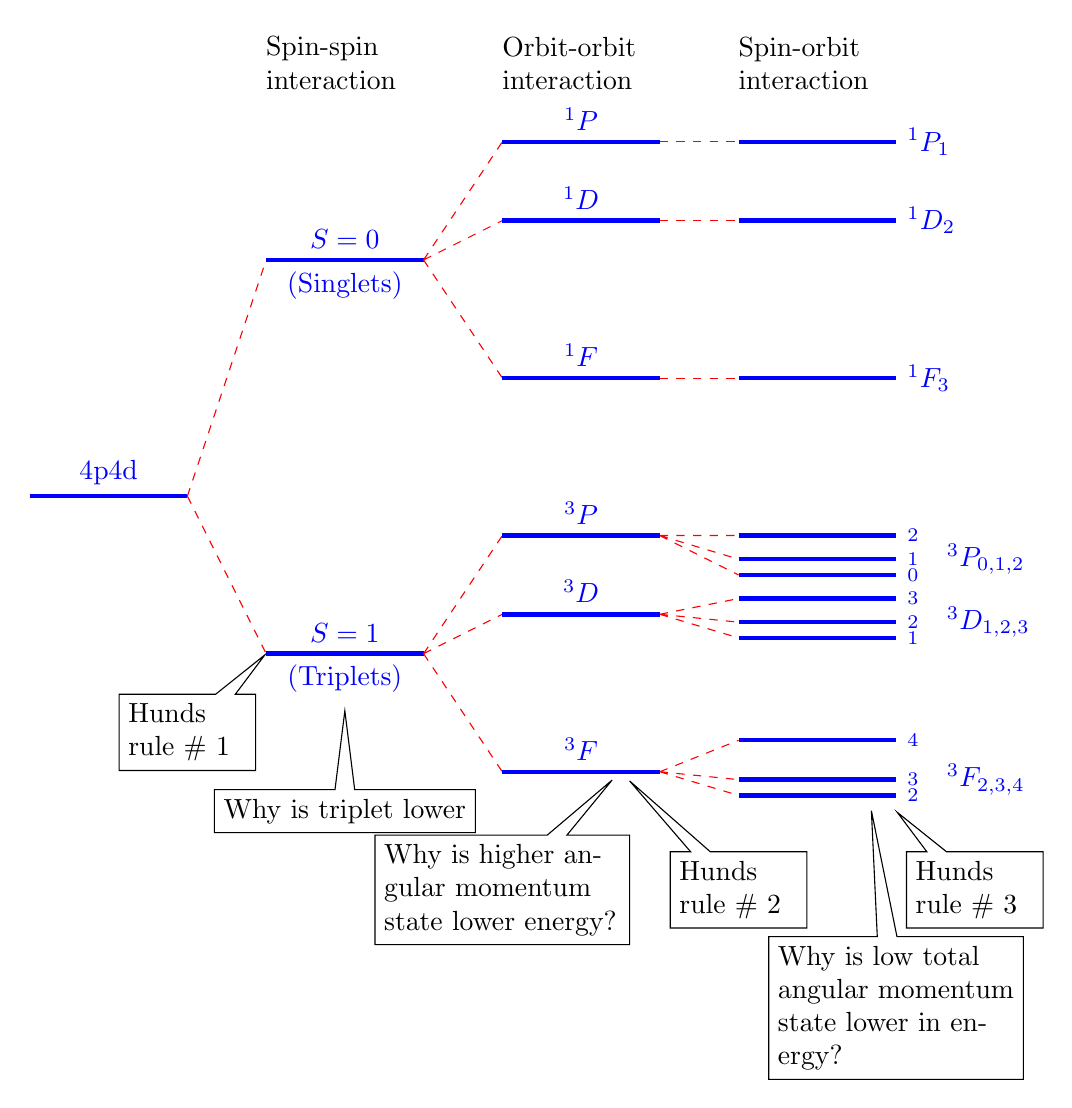
\begin{tikzpicture}
   % Draw all levels
  \draw[level] (0,0) -- node[above] {4p4d} (2,0);

  \draw[connect] (2,0)  -- (3,-2) (2,0) -- (3,3);
  \draw[level]   (3,3)  -- node[above] {$S=0$} node[below] {(Singlets)} (5,3);
  \draw[level]   (3,-2) -- node[above] {$S=1$} node[below] {(Triplets)} (5,-2);

  \draw[connect] (5,3)    -- (6,4.5) (5,3) -- (6,3.5) (5,3) -- (6,1.5);
  \draw[connect] (5,-2)   -- (6,-0.5) (5,-2) -- (6,-1.5) (5,-2) -- (6,-3.5);
  \draw[level]   (6,4.5)  -- node[above] {${}^1P$} (8,4.5);
  \draw[level]   (6,3.5)  -- node[above] {${}^1D$} (8,3.5);
  \draw[level]   (6,1.5)  -- node[above] {${}^1F$} (8,1.5);
  \draw[level]   (6,-0.5) -- node[above] {${}^3P$} (8,-0.5);
  \draw[level]   (6,-1.5) -- node[above] {${}^3D$} (8,-1.5);
  \draw[level]   (6,-3.5) -- node[above] {${}^3F$} (8,-3.5);

  \draw[connect] (8,4.5) -- (9,4.5) (8,3.5) -- (9,3.5) (8,1.5) -- (9,1.5);
  \draw[level]   (9,4.5) -- (11,4.5) node[right] {${}^1P_1$};
  \draw[level]   (9,3.5) -- (11,3.5) node[right] {${}^1D_2$};
  \draw[level]   (9,1.5) -- (11,1.5) node[right] {${}^1F_3$};

  \draw[connect] (8,-0.5) -- (9,-0.5) (8,-0.5) -- (9,-0.8) (8,-0.5) -- (9,-1)
                 (8,-1.5) -- (9,-1.6) (8,-1.5) -- (9,-1.8) (8,-1.5) -- (9,-1.3)
                 (8,-3.5) -- (9,-3.8) (8,-3.5) -- (9,-3.6) (8,-3.5) -- (9,-3.1);
  \foreach \i/\j in {2/-0.5, 1/-0.8, 0/-1} {
    \draw[level] (9,\j) -- (11,\j) node[right] {\scriptsize $\i$};
  }
  \node[level, right] at (11.5,-0.8) {${}^3P_{0,1,2}$};
  \foreach \i/\j in {3/-1.3, 2/-1.6, 1/-1.8} {
    \draw[level] (9,\j) -- (11,\j) node[right] {\scriptsize $\i$};
  }
  \node[level, right] at (11.5,-1.6) {${}^3D_{1,2,3}$};
  \foreach \i/\j in {4/-3.1, 3/-3.6, 2/-3.8} {
    \draw[level] (9,\j) -- (11,\j) node[right] {\scriptsize $\i$};
  }
  \node[level, right] at (11.5,-3.6) {${}^3F_{2,3,4}$};

  % Draw labels
  \node[label] at (4,5.5)  {Spin-spin interaction};
  \node[label] at (7,5.5)  {Orbit-orbit interaction};
  \node[label] at (10,5.5) {Spin-orbit interaction};

  % Draw annotations
  \node[notice={(0.5,0.5)}, text width=1.5cm] at (2,-3) {Hunds rule \# 1};
  \node[notice={(0,1)}] at (4,-4) {Why is triplet lower};
  \node[notice={(0.7,0.7)}, text width=3cm] at (6,-5)
    {Why is higher angular momentum state lower energy?};
  \node[notice={(-0.9,0.9)}, text width=1.5cm] at (9,-5) {Hunds rule \# 2};
  \node[notice={(-0.2,1.6)}, text width=3cm] at (11,-6.5)
    {Why is low total angular momentum state lower in energy?};
  \node[notice={(-0.5,0.5)}, text width=1.5cm] at (12,-5) {Hunds rule \# 3};
\end{tikzpicture}
\end{document}
